\chapter{Introduction to Information}

%\textit{``Anything worth knowing is worth writing down"}
%bullseyed723 (reddit.com 2016)

\begin{flushright}
    \textit{``Who among you can laugh and be elevated at the same time?''}
    \\ --- Friedrich Nietzsche
\end{flushright}

This thesis contains much more social and theoretical analysis than is typical of an information science thesis, especially in these earlier chapters. Very quickly, however, we will move on to the literature review and empirical research with practical applications.

The previous chapter (Chapter 1) made the case that access to information should be a fundamental human right. This chapter concerns the history of information; a brief chronology accounting for its place in human culture and how our ancestors created, shared, and destroyed information and concludes by discussing if our modern information systems are any better. Chapter 3 explains modern information retrieval systems (search engines). Chapter 4 covers written language as the primary medium used by search engines; introducing many linguistic concepts which will be used in our experiments. Chapter 5 covers linguistic methods used to improve a user's search query, primarily query expansion. Chapter 6 outlines the experimental conditions, which include a search engine, a data set of search queries, and a linguistic ontology. Chapter 7 and Chapter 8 each propose novel improvements to query expansion, specifically addressing the problem of query drift. Chapter 9 discusses the limitations of our experiments. Chapter 10 concludes the thesis with some thoughts on why natural language processing can be such a difficult task.

The original research question was: can we improve search engines? This thesis answers a more specifc research question: can we measurably mitigate the query drift caused by query expansion? Spoiler alert! the answer is: yes. However, it's probably best to avoid causing query drift to begin with.

\section{A Brief History of Information}

The second half of the second decade of the third millennium is in the midst of the digital information age and has been for my whole life. The entire collective wisdom of humanity is readily available to everyone through the information superhighway. Notable exceptions of this triumph of humanity are given to the Amish, members of the Gloriavale commune, high-risk offenders, North Koreans, and the uncontacted tribes of the Andaman Islands. It does seem politically incorrect to equate religious fundamentalists with criminals, a totalitarian kleptocracy, and pre-agricultural civilisation... but it is factually correct. I sincerely believe that the primary directive of information retrieval is to facilitate access to \textit{all} information for every living person on earth... even if it does breach The Prime Directive.

The technology used to represent information has advanced substantially across the millennia of human history, from pictograms of aurochs scrawled onto the surface of palaeolithic cave walls (Figure \ref{fig:cave}) to a digital motion-picture (Figure \ref{fig:picasso}) beamed at the speed of light from a solid-state drive in Google's Datacenter through an optical fibre submarine cable crossing the Pacific Ocean, all the way from the west coast of the North American continent to New Zealand, down the South Island's backbone, through a complex network of exchanges, routers, and switches, entering my computer's CPU at the speed of light, causing trillions of transistors to switch billions of times every second to magically transform this cross-continental signal into a video of Picasso painting a Bull, or otters holding hands, or a panda sneezing.

We are truly Gods, beyond the imaginings of our past selves.

\begin{figure}[!tbp]
  \begin{subfigure}[b]{0.49\textwidth}
    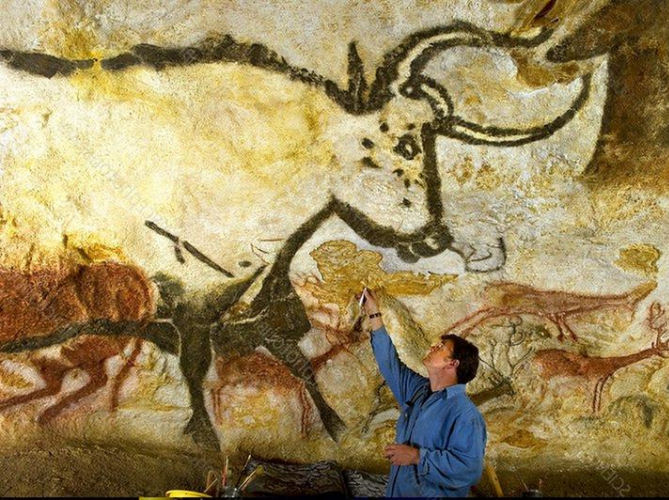
\includegraphics[width=\textwidth]{graphics/bull_cave.jpg}
    \caption{Cave Painting.}
    \label{fig:cave}
  \end{subfigure}
  \hfill
  \begin{subfigure}[b]{0.49\textwidth}
    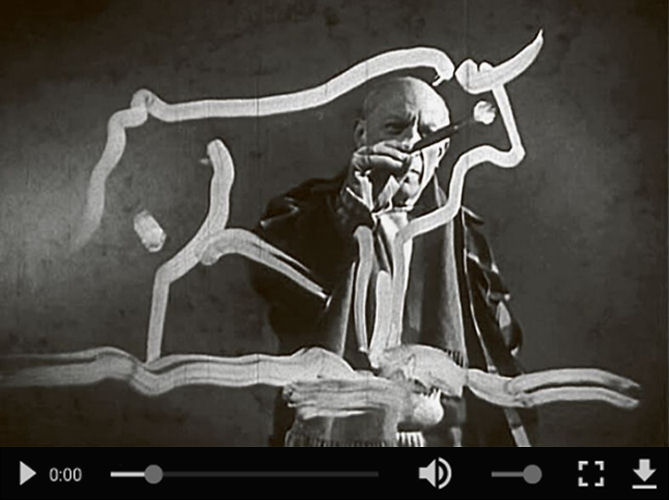
\includegraphics[width=\textwidth]{graphics/bull_picasso.jpg}
    \caption{YouTube Video.}
    \label{fig:picasso}
  \end{subfigure}
  \caption{Information does not change, but the format clearly does.
  \\(a) Restoring `Great Hall of the Bulls', painted by humans 17,000 years ago.
  \\(b) Pablo, in the documentary `Visite à Picasso', painting a bull 71 years ago.}% \url{https://youtu.be/W3pfNT6qJUk.}}
  \label{fig:bull}
\end{figure}

\section{The Birth of Books}

A picture may be worth a thousand words, but language is our primary format for information. Archaeology tells us, it was during the Bronze Age when we first attempted to ensconce wisdom from the storytelling tradition into a permanent written record. Information on parchment and papyrus survived for a thousand years or more, far beyond the 34-year life expectancy of palaeolithic humans\footnote{\url{https://doi.org/10.1002}}. Writing as technology was cheaper, easier, more portable, and more space economical than stone carvings. These extant documents include: \textit{The Epic of Gilgamesh, Rig Veda, I-Ching, Brahmana, The Torah, Homer's Odyssey, Bhagavad Gita} and \textit{Aesop's fables}. These codified oral accounts are famously poetic, as they were designed to be memorized. The rhythm and rhyme help preserve plotline for a much longer time. 

These documents were written during a time when our primitive understanding of causality led us to believe that a certain dance would cause rain to fall, stabbing a doll that resembled our enemy would inflict actual pain, and uttering a curse would rouse the wrath of God(s). This faulty logic is what we would now call ``magical thinking''. These thoughts reinforced by correlated events. Rainfall is inevitable regardless of any prior dancing, but if you always perform a special dance during a drought, then the eventual post-drought rain will always come to pass after your dance.

The smug atheist of today considers these significant documents as mere apocryphal stories, fantastical fairy-tales, theological, and mythical in nature... which is not untrue, but it detracts from the facts... these are our early attempts at understanding our world. These are sincere attempts at academic scholarship that we now call: \textit{History, Astronomy, Meteorology, Mathematics, Natural Science, Medicine, Cosmology, Psychiatry, Ethics, and Metaphysics}. Many ancient observations recorded as facts remain facts to this day: trees grow tall, birds fly higher, and love is all-powerful. However, these documents also contain the pseudo-scientific-mumbo-jumbo that we now call: \textit{Numerology, Naturopathy, Acupuncture, Karma, Reincarnation, Spiritual Ascension, Witchcraft, Voodoo, Baptism, Prayer} and other occult practices. Many are provably unharmful but also provably ineffectual, so they are often practised under the divine blessings of \textit{Placeboeffectus}, the trickster god of quackery and fraud. 

Trying to extract moral wisdom or even useful information from these ancient documents is difficult, as they were written before the pursuit of knowledge had matured into a rigorously reliable artform. Over the past couple thousand years, we have developed: Skepticism, Empiricism, Rationalism, Verificationism, Disinterestedness, and Falsifiability, crucial skills needed to sculpt pristine sculptures of understanding from the messy muck of reality.

\section{The Greeks Wrote Books}

Today, people take great pride in the number of books they have read, which is a recent trend as for the majority of human history, nobody was expected to be widely read. Even academic scholars read a measly pittance of books, but they read them well, and they read them often. This is clear when considering religious cultures: the Muslim's Qu'ran, the Jew's Torah, the Hindu's Bhagavad Gita... Even the good citizens of Ancient Greece were expected to know Homer's Odyssey and The Iliad. These were not just epic tales; they were comprehensive compendiums of wisdom, teaching courage, kindness, honesty, and justice. 

Greek wisdom survives through these Ancient Greek Myths, different from Modern Greek Myths, like the long term sustainability of national debt. The secular wisdom and philosophy of the Ancient Greeks form the structural foundation of western civilization. The most famed philosophers are the big three. \#1: Socrates, who gave us the examined life, the interrogative method, and he also taught \#2: Plato, who formalised justice and ideas, and he taught \#3: Aristotle, the first aristocrat\footnote{Strictly in a linguistically non-anachronistic sense.} and polymath, the most influential of the three as he wrote the most prolifically. He is credited with dividing worldly knowledge into the disciplines that persist to this day: \textit{Physics, Biology, Mathematics, Ethics, Politics, Art, Poetics...} Although not everything Aristotle wrote is revered; he propagated the geocentric solar system, that slavery is necessary, that the speed of falling objects is proportional to mass, and that women are the inferior sex: as they are passive, more deceptive, complain more, and have fewer teeth!\footnote{I too would complain more if Aristotle accused me of inferiority after undercounting my teeth.}

From this era survives the work of countless great thinkers: Pythagoras, Zeno, Euclid, Archimedes, Eratosthenes, and my two favourites Epicurus and Diogenes of Sinope. Along with the invention of writing, the other major catalyst for the information boom of Antiquity was the invention of currency. Money facilitated individuals to accrue wealth, allowing them to spend less time toiling and more time writing. Currency was not an isolated incident; it spread fast, giving rise to cross-continental merchant trade. The Silk Road united the span of Eurasia; from the West to the East, there were massive escalations in book learning. In the East, this period of history is known as the \textit{Hundred Schools of Thought}, as there were so many thoughts being taught. The most influential thinkers were: Confucius, founder of Confuciusm; Buddha, founder of Buddhism; Sun-Tzu, author of The Art of War; Laozi, author of the Tao-Te-Ching; and the apocryphal man Zarathustra, who \textit{spake thusly}. The thinkers in Persia, India, and China existed simultaneously but largely independently of the Ancient Greeks. While fine silks, wealth, and disease managed to traverse the chain of merchants across the breadth of Eurasia, scholarly information did not, largely because of the cascade of language barriers but also because commercialising ideas directly was not feasible. Thankfully patent law fixed this problem until patent trolls ruined it.

\section{The Romans Burned Books}

Greek thought began to spread across the Mediterranean after Aristotle's student, Alexander the Soon-to-be-Great, decided that Greece was a bit too small and not enough people spoke Greek, so he began a campaign of murder until everyone else agreed. Following Alexander's example, everyone else really wanted to have a go at global domination, and for a few centuries, the Mediterranean was consumed with murderous warfare. During this period, vast swathes of literature were lost, science, philosophy, poetry, incidentally destroyed as military generals burned cities in conquest. 

The Platonic Academy was destroyed by the Roman dictator Sulla during the Siege of Athens in 86 BC, 38 years later in 48 BC (this was back when we counted backwards) the Great Library of Alexandria was burned, likely by the Roman dictator Caesar during a military invasion. The Great Library of Alexandria was one of Antiquity's most significant research institutes; it held approximately 100,000 books and scrolls. All of them were destroyed during a military invasion, a fitting end to a library indirectly named after Alexander the Great, the man famed for military invasion.

The Roman Republic, triumphant in warfare later succeeded by the Roman Empire, held sovereignty over the West. After they decimated most of Greek culture, the Romans then appropriated what was left: Zeus became Jupiter, Democracy became Imperialism, Shipbuilding became Road building, slavery remained slavery, and wine remained wine.

\section{The Christians Burned Books}

Around this time, some whippersnapper called Jesus started preaching love, forgiveness, and magic tricks. He said killing was not groovy, so they killed the proselytising raconteur and occult magician. In the following couple of centuries, Christianity was outlawed in Rome. If alcohol prohibition has taught us anything it is that activities become infitely more appealing when outlawed and you cannot stop people using their bathtubs to make moonshine and bootleg baptism. The clandestine Christian movement reached a tipping point in 313 CE when Emperor Constantine proclaimed Christianity legal in the Edict of Milan. In 380 CE, Emperor Theodosius proclaimed other religions heresy in the Edict of Thessalonica, and encouraged the people to inflict the \textit{will of heaven} onto the heretics. By 400 CE, the Roman Empire was in rapid decline, and the rise of Christian dominance was in full swing.

Unfortunately, the early Christians were responsible for far more destruction than the Roman's were. They deemed most scholarship heretical and morally corrupt, as little of it credited God directly. They purposefully burned books, not as an unfortunate byproduct of war, but with malevolent intent, they defaced books and paintings, smashed statues and temples of education, in a repugnant display of viciously violent fanaticism. From the ashes of the Greco-Roman world arose churches of worship; Philosophy and science were replaced with scripture and reverential poetry. Worse still, under the oppression of Christian orthodoxy, fewer books were published, progress was stifled, education of the masses waned in favour of blind, ignorant dogma.

What the early Christians started, the Goths, Huns and Vandals continued. Centuries of progress was irretrievably lost, with religious zealots largely to blame. Some estimate that as much as 90 percent of the literature of antiquity was lost \cite{rohmann2016christianity}. Most of our knowledge of Antiquity survives through partial fragments, brief summaries, and later commentaries. Less than a quarter of Aristotle's works survive\footnote{\url{http://www.rmki.kfki.hu/~lukacs/ARISTO3.htm}}. Most other scholars were not as lucky; the Epicurean philosophy of happiness persisted as a popular lifestyle for centuries until Christianity deemed it heretical. And of Epicurus's 300 works, almost nothing survived, and it's still more than most \cite{kenny2010new}. 

How crippled would our future society be if the works of Shakespeare, Newton, Einstein and Freud were lost today? This was a dark end; religious extremists, power hunger warlords, and sadistic barbarians irretrievably destroyed almost every god damned thing.

\section{The Muslims Saved Books}

The 1,000 year period between the fall of Rome, and the rise of the Renaissance, between the 5th century CE and 15th century CE, was a dark time. Under feudalism, cultural and economic deterioration plagued us, as did actual plagues. We call this era the Dark Ages or Middle Ages... however, the Middle East calls this era The Islamic Golden Age. My Anglo-Christian education failed to inform me of this information boom. 

At the heart of this era was the House of Wisdom in Baghdad, a library that homed academics who rivalled the Ancient Greeks and preempted much of Renaissance philosophy. After the Prophet Muhammad wrote the Qur'an, the Lexicographer Al-Khalīl wrote the first dictionary. While one of these books was taken as gospel, the other was an actual significant human achievement. Mathematician Al-Khwarizmī ---Father of Algebra--- revolutionised Algebra, Arithmetic and Trigonometry with the bleeding edge technology of Hindu-Arabic numerals. Polymath Avicenna wrote \textit{``the''} textbook on medicine which prevailed until the 19th century CE. His \textit{``flying man"} thought experiment explicated the mind-body duality that the Christian philosopher Descartes repeated 600 years later with \textit{``Cogito Ergo Sum"}. Why does Descartes get the credit? Philosophy is Groundhog Day, and language barriers between cultures impinge progress. Most importantly, the Islamic scholars of this era recovered some books from Ancient Greece... they translated these works, wrote commentaries, built upon them, adopted their ideas, which unfortunately included much of Aristotle's misogynistic opinions, which were used to defend their own misogynistic practices: like a pre-millennium Christian using the Bible to defer the blame of their own rampant homophobia. However, the foundation of modern scholarship rests on Aristotle's shoulders, and if they had been lost, our progress could have been set back centuries, so we thank our Islamic ancestors. 

Unfortunately, history repeats itself. In 1258 CE Baghdad was sieged, The House of Wisdom and its contents were destroyed, the Mongols were to blame, lead by the notorious Genghis...

\begin{center}
\textit{``KHAAAN!!!!''}\\ --- Admiral James T. Kirk
\end{center}

\section{The Europeans Refined Books}

Thankfully, not all was lost. Another era of information began when Catholic scholars rediscovered Aristotle (from Islamic commentary) around 1200 CE, 15 centuries after Aristotle's death. Fibonacci reintroduced and popularised the Arabic-Hindu number system; Thomas Aquinas gave us Scholasticism; William of Ockham gave us Ockham's razor, and Duns Scotus gave use the pejorative \textit{``Dunce''}. Unfortunately, this rising force of scholastic scholarship ended abruptly in 1346 CE with the Black Death, the largest population decimation in human history, taking a mere four years to kill half of all Europeans, faster even than COVID eradicated Trump supporters.

Across the globe, there have been many information booms, separated by information winters, caused primarily by warfare, disease, and the bigotry of the religious. It was not until the mechanical printing press was developed in the mid 15th century (1440 CE) that an information boom could permanently take hold, as books could be produced at a rate significantly faster than they could be destroyed.

% The 16th century saw the Renaissance (1494 – 1550) 
% The 16th-17th century saw the Scientific Revolution (1543 – 1687)
% The 18th century saw the Age of Enlightenment (1715 – 1789)  
% The 18th-19th century saw the Industrial revolution (1760 – 1840)

% At the tail end of the industrial revolution started the science and inventions 

% 1833 Science as a profession, "scientist" meaning Knowlegde Artist is invented
% 1959 Darwin's natural selection
% 1861 Maxwell formulates the four Maxwell equations
% 1873 Maxwell published treatise of Electromagnetism

% 1856 Louis Pasteur discovers Pasteurisation
% 1875 Alexander Graham Bell's telephone
% 1879 Thomas Edison's practical incandescent light bulb.
% 1879 Louis Pasteur's laboratory developed vaccine.
% 1885 Louis Pasteur's developed rabies vaccination.
% 1888 drinking straws
% 1890 cardboard box
% 1891 electric kettle
% 1901 vacuum cleaner
% 1903 the teddy bear

The rest of the Scientific Revolution is well known here in the west; we tend to wear our Anglocentric knowledge on our smug sleeves, we keep it right next to our ignorance of other cultures. Francis Bacon gave us The Scientific Method. Galileo fought religious opposition for heliocentrism after Copernicus failed to. Newton, Descartes, Kepler, Leibniz, Spinoza, Pascal, Shakespeare, Locke... all thinkers in the same generation that were not lost, most notably Gutenberg himself, who invented the machine that literally immortalized his name. Followed closely by Voltaire, Euler, Hume, Kant, Rousseau, Watt, Gauss, Darwin, Schopenhauer, Hegel, Schelling, Kierkegaard, Spencer, Freud, Hilbert, Twain, Nietzsche, Planck, Curie, Jung, Einstein, Schrodinger, Wittgenstein, Heidegger, Koestler, G{\"o}del, Turing, Grice, Camus, Feynman, von Neuman, Tesla, Austin, Lacan, Popper, Foucault, Derrida, Sagan... a never ending list, but dominated largely by German men (i.e. citizens of the Holy Roman Empire 2.0).

%Industrial revolution 

%16th Century saw the rise of mass production of books, after the advent of the printing press in the

%12th Century saw the rise of manuscript production

%previous to that was the codex manuscript, which were hand written by authors, and hand written by scribes.

%Wars are driven by economic and political reasons, a greedy desperation for resources, which is unsurprising in a society largely dependent on resources.

This simplified narrative above, the history of information, is pieced together from extant documents. It's incomplete because it leaves out precisely what has not survived, including even what we are unaware of what has not survived. If you doubt any part of this historical timeline you can check Wikipedia as a source of truth, I know it's all on there because I put it there myself. 

I would argue that the greater loss of war is not human life but rather the irreparable loss of information itself. The life of any individual is highly overrated. Death cannot be prevented, only delayed. However, we can prevent the death of information. Information can be immortal, and helping information achieve immortality for our future generations could be humanity's greatest achievement. 

%Historical humanity goes through cycles of information revolution, the rise of scholarship followed by irreversible destruction. The extents of knowledge 



%The myth of Jesus has value, as the myth is immortal, it outlived the man himself.

%The first historical account I've ever seen that doesn't use glorify military commanders, and political leaders... the kinds of people who not only think they can change the world, but also openly claimed to want to change the world... which is just claiming to look marvelous in statue form\footnote{Why is Alexander the Great considered a brilliant military commander, and it's only Hitler and Stalin we call evil. Alexander the Great? more like Alexander the Sycophantic Cunt... war mongering, blood lusting, missionary of death. I wish he was brutally tortured and mutilated as a child, in-order to simultaneously in-act retroactive justice and prevent his serial-killing-spree. And even worse, I wish him forgotten, it's too late, his name is immortal.}.

\section{The Obsolescence of Books}
This brings us to the latest information era, the era of digital information, which started around the birth of the world wide web, a few years before my own birth. We now have an interconnected network of digital Information systems which have heavily changed almost every aspect of our lives, in both trivial and significant ways. It has affected commerce, politics, education, mass surveillance, and most notably in the acquisition of pornography. It's also responsible for an abundance of misinformation and disinformation, like political propaganda, vaccine scepticism, and the Berenstein conspiracy. Such extravagant information replication and proliferation would not be possible with the antiquated paper system of antiquity or word of mouth before that, which is fantastic! As I sincerely believe in unrestricted freedom of information. I cannot fathom a good reason why any knowledge should be forbidden or censored, for when it is, there immediately becomes a sectarian divide between those who know and those who do not, an imbalance that can be used to exploit and manipulate. Even if dissenting ideas are seen as vulgar, objectionable, or spark controversy, they should still be openly shared because there cannot be progress without direct confrontation of controversy. If everyone agrees with the status quo, the status quo will persist long after its expiry date.

\begin{center}
\textit{``I may not agree with you, \\but I will defend to the death your right to make an ass of yourself.''} \\ --- Oscar Wilde
\end{center}

The impressive immediacy of information transmission the internet allows should only increase the rate of progress. However, it is not soley my responsibility to fully explicate the ethics of digital information. I will leave the rest of the proof as an exercise for the reader. My primary ambition is to improve the platform that distributes information. It is, however, an immutable fact that there is an abundance of knowledge, more than ever in human history, directly at our fingertips. Information Retrieval directly mediates our access to almost all of this information, from the carefully constructed digital libraries of academia, arts and science, to the vast open plains of the world-wide-web, and the underbelly of the darknet (e.g.\ page three of Google). But despite the technological prowess modern internet search engines claim to have, I am still unable to find a serious meaning in the TV series finale of Lost or find a good reason as to why banks are unable to transfer digital currency between databases on a Sunday. There is obviously much progress to be made... the truth is out there!

\begin{center}
    \textit{``Scientia potentia est"} (knowledge is power) 
    \\ --- Francis Bacon
\end{center}

It's widely believed that having knowledge gives you power, which it does, but more than that, knowledge itself \textit{is} power, and humanity is directly subservient to it. We are dedicated to the pursuit of knowledge, and our livelihood depends on knowledge, but it does not depend on us. The essentialist's knowledge exists independently from us; only our own awareness of knowledge depends on our own existence. We willingly search it out, increasing our awareness of it, stacking it up into teetering towers of unread books, filling halls of libraries, gathering dust to symbolise our collective knowledge despite individual ignorance.

What is the difference between knowledge and information? Some say \cite{lucky1989silicon} that there is a hierarchical relationship between wisdom, knowledge, information and data, which is thus:

\begin{center}

Data $\Longleftrightarrow$ Information $\Longleftrightarrow$ Knowledge $\Longleftrightarrow$ Wisdom

\end{center}

There is heaps of data on the net, and provided our perception of time appears to be unidirectional, the amount of data will not reduce (Assuming bureaucrats do not burn the Internet). We have managed to amass thousands of years of culture, art, science, technological development, and photographs of spiralized courgettes served on toasted pumpernickel at upmarket high street cafes tagged unironically as \textit{\#bourgeoisie} on Instagram. And many of us humans have an urge to retain all of this \textit{``stuff''} for the future benefit of future peoples, for the prosperity of posterity, for nostalgia, and oftentimes... just `coz.

%%%%%%%%%%%%%%%% DATA
\textbf{Data} can be recorded from almost any source. We can even algorithmically generate any arbitrary piece of data. All we need is a surplus of immortal monkeys and unbreakable typewriters to generate anything, the majority of which would be worthless noise. This kind of data is noise; it has no meaning or practical usefulness. However, the information content could be quite high, as uniform-random data has high entropy due to its lack of predictability.

%%%%%%%%%%%%%%%% INFORMATION
\textbf{Information} is data with a provided context; it has some meaning and practical usefulness. We measure information content by its predictability, not by its perceived importance or usefulness. This leads us to the counter-intuitive notion that uniform-random noise contains more information than deliberately structured information. The imposed structure on data provides predictability through redundancies (assuming uncompressed data), e.g.\ for a document written in the English language (part of the context), a \textit{`q'} is very likely to be followed by a \textit{`u'}, even if it is written on a QWERTY keyboard by a Qantas pilot flying to Qatar. The difference between the white noise received on a near-obsolete FM radio and a .mp3 of \textit{``A Candle in the Wind"}; the difference between the echo of the Big Bang's background radiation received through a UHF antenna and a .mov of a cat playing the piano.

%%%%%%%%%%%%%%%% KNOWLEDGE
\textbf{Knowledge} is a wider concept than information; it takes into account the full breadth of the information's context. It describes the connections between pieces of information because facts do not exist independently floating in a void but rather within an interconnected network. A collection of related pieces of information is called a knowledge base or an ontology—an intricately structured model categorising things and their associated relations. A popular model for a digital knowledge base is the Resource Description Framework, representing associations as edges within a directed multi-graph. The great thing about these kinds of knowledge bases is that you can deduce new information by following a chain of inferences, which is far more difficult to do with Relational Databases or Associative Key-Value-Pair Maps.

%You will have already used one of these systems, Google's Knowledge Graph, which is invoked during every web search, and the results are shown in the infobox on the right. 

I assume that all knowledge is perilously close to assumption. Any inference exists on a spectrum between a justified deduction from all the readily available evidence and a bigoted generalization. This is because any knowledge base (digital or mental) is incomplete and full of inaccuracies. Any good knowledge base is not temporally static. It acquires new information and corrects itself over time. Knowledge is rarely consistent. There are frequent exceptions, caveats and contradictions, making it impossible to be certain about almost anything. However, biological minds can still make material inferences and predictions about our reality through an intuitive approach, an enigmatic fuzzy-logic\footnote{Some might say faulty cognitive heuristics.}, rather than a strictly rational system. Our minds have the ability to extract the information from our experiences into ordered schemata and patterns of association, generalisations from which we can intuitively infer. This is why when I was four years old, I told Mum, \textit{``I don't want long hair because I don't want to be a girl.''}. This does not mean the pursuit of truth is futile, but it is important to maintain the clarity of the epistemological hierarchy at all times.

%human communicaiton works on assumption and inference.
%indirect speech (implicature, entailment, likelihood disambiguation, presupposition, shared mutual knowledge...)
%Conversation is a cooperative act
%both participants excert cognitive 

%%%%%%%%%%%%%%%% WISDOM
\textbf{Wisdom} is based on the practical application of knowledge and entails either an individual or collective belief in its perceived validity. I can say \textit{``The chicken came before the egg"}, which is definitely a piece of knowledge\footnote{Especially if one trusts Genesis 1:20-22}, but whether it is universally accepted as truth is contentious, and whether it is useful is unclear. 

Here's a more serious example, proverbial wisdom I hear often:

\begin{center}
\textit{``Reliance on digital media is corrupting the youth of today."}
\\ --- Conventional ``boomer'' Wisdom
\end{center}

This is definitely data; there's an informational context; it is relevant and strongly associated with many aspects of my (and your) contemporary lifestyle. But is it wisdom? Is it wise to live our lives by it? Only time and God can tell. And since I can hear neither time nor God, let's contrive a prophecy!

We know that historically the introduction of other forms of media caused widespread scepticism and, in many cases, mass panic. When television became popular, there was fear that we would never talk to each other; we would stare at the fluorescent screens like zombies; there would no longer be a conversation over the dinner table ever again. Telephones were also thought to end the family's chat-chat as the phone's ring would draw attention away, attention spans would be disrupted because you would be constantly interrupted. Going back even further, to when writing became hip in Ancient Greece, literacy was considered by many to be degenerate and decadent, and your memory was expected to deteriorate due to neglect. There was a genuine fear that people would not cultivate their memory since one could write everything down and lazily refer to it later. Now since you are likely reading this sentence in print, I shall refrain from convincing you of the value of literacy; you're already part of the system, it's too late for you.

I would not claim that digital media is all pristine peaches and refined roses, but the benefits surely outweigh any detriments by orders of magnitude. So it stands to reason that fearing the rise of digital media is merely unfounded speculation, which is in line with the human tradition of delusional mass panic. The uncertainty of the future is certainly frightening; we have no assurance that anything will be O.K.\footnote{O.K. a joke from the 1840s, an ironic misspelling of \textit{All Correct} (\textit{Oll Korrect}).}. The existential malaise is omnipresent. It's natural to justify this fear by contriving an argument against the unknowable effects of digital media or some other new-fangled technology. Because there is no genuine prophetical oracle, there cannot exist any certain affirmations that would dissuade the conservative pessimists that plague progress. But with patience, time will prove wrong the negative Nancy's and doubting Thomas's who fight progress, as it has done, again and again and again. I, for one, do not mourn the loss of the hunter-gatherer jobs that were lost during the rise of agriculture.

%The future is by virtue of itself uncertain, the past however is 
%fondly nostalgical
%it's certainty is reassuring

%It takes courage to venture into the future, in fact you can't be courageous without fear.

%technological obsolescence
%I for one do not mourn the loss of the hunter-gatherer jobs that were lost during the rise of agriculture
%I refuse to light my home with electric light bulbs, support the candle industry! 
%I refuse to use photocopiers, support the scribe industry!

%The long-term goal of any society should be complete unemployment

%I do not understand the obstinate refusal to stand on the shoulders of giants

That was supposed to be wisdom, of a polemic flavour, centrally about the value of digital media and information retrieval. The point is, we should rejoice, as it appears there are more signs that our society is heading towards a Star Trek utopia, not a Mad Max dystopia. The next chapter explains how modern search engines work, and we will also begin the enquiry into what prevents clear communication between information retrieval systems and their users.
